\section{The Meissner Effect}
Another truly remarkable property of superconductors is its electromagnetic properties, which are radically different from those of metals.
Inside a metal, we have $\vb E = 0$. However, an externally applied magnetic field $\vb B$ will essentially penetrate a metal completely

\begin{figure}
	\centering
	\begin{subfigure}{0.45\textwidth}
		\centering
		\begin{tikzpicture}
	\draw[fill, blue!50!gray, opacity =0.5] circle (1.3cm);
	
	\foreach \x in {-1.5,-0.5,0.5,1.5}
	{
		\draw[very thick,->-=0.5] (\x,-3) to (\x, 3);
	}
	\node[anchor= west] at (1.5,2){$\sim \vb B$};
\end{tikzpicture}
		\caption{$T>T_C$ (metal)}
		\label{fig:meissn_a}
	\end{subfigure}
	\begin{subfigure}{0.45\textwidth}
		\centering
		\begin{tikzpicture}
	\draw[fill, blue!50!gray, opacity =0.5] circle (1.3cm);
	
	\coordinate (a) at (-1.8,0);
	\coordinate (b) at (-1.5,0);
	\coordinate (c) at (1.5,0);
	\coordinate (d) at (1.8,0);	
	
	\draw[very thick, ->-=0.5] (-1.5,-3) to[out = 90, in = -90] (a);
	\draw[very thick, ->-=0.5] (-.5,-3) to[out = 90, in = -90] (b);
	\draw[very thick, ->-=0.5] (1.5,-3) to[out = 90, in = -90] (d);
	\draw[very thick, ->-=0.5] (.5,-3) to[out = 90, in = -90] (c);
	
	
	\draw[very thick, ->-=0.5] (a) to[out=90, in=-90] (-1.5, 3);
	\draw[very thick, ->-=0.5] (b) to[out=90, in=-90] (-.5, 3);
	\draw[very thick, ->-=0.5] (d) to[out=90, in=-90] (1.5,3);
	\draw[very thick, ->-=0.5] (c) to[out=90, in=-90] (.5,3);
	
	
	\node[anchor= west] at (1.5,2){$\sim \vb B$};
\end{tikzpicture}
		\caption{$T<T_C$ (cooled before applied magnetic field)}
		\label{fig:meissn_b}
	\end{subfigure}	
	\caption{Meissner effect.}
	\label{fig:meissner_1}
\end{figure}
If there is any tendency for the system to resist admitting the external $\vb B$-field, then this is called \underline{diamagnetism}. In a metal ($T>T_C$) this diamagnetism is very \underline{weak}, see \cref{fig:meissn_a}. In a superconductor ($T<T_C$) this is very different. If we take a metal and cool it down and then apply an external field, the magnetic field is excluded, as shown in \cref{fig:meissn_b}.


Now, the magnetic field is entirely excluded from the superconductor. This is called the \underline{Meissner-effect}. 
We will now relate the Meissner-effect to the onset of a gap $\Delta_k$ below $T_C$. 
\begin{tcolorbox}
	The Meissner-effect is the essential phenomenon characterizing a superconductor.
\end{tcolorbox}
Start with the Maxwell-equations relating magnetic field to a current $\vb J$.
\begin{align}
	\div{\vb B} = 0 &\implies \vb B =\curl{\vb A} \\
	\curl{\vb B} &= \mu_0\vb J	
\end{align}
Now, as always, we need a constitutive relation for the current $\vb J$. Obviously, the standard one, $\vb J = \sigma \vb E$, where $\sigma$ is conductivity and $\vb E$ is electric field, will not work, since it gives Ohmic resistance.

Supercurrent:
\begin{equation} 
\vb J_s = e^*n_s\vb v_s.
\end{equation}
\begin{enumerate}[]
	\item $e^*$: An effective ``quasiparticle'' charge
	\item $n_s$: density of superconducting charge-carriers (Bogoliubov quasiparticles)
	\item $\vb v_s$: velocity of such quasiparticles
	\item $\vb v = \frac{\vb p}{m^*},\quad m^*$: Mass of quasiparticle.
\end{enumerate}
In the presence of an electromagnetic field,
\begin{align} 
\vb p &\rightarrow \vb p - e^*\vb A\\
\vb J_s &= \frac{e^*}{m}n_s\left( -e^*\vb A \right) = -\frac{\left(e^*\right)^2}{m}\vb A \\
\curl{(\curl{\vb A})} &= \mu_0\vb J_s = -\frac{\mu_0\left( e^* \right)^2n_s}{m}\vb A\\
\curl{\left( \curl{\vb A \right)}} &= \grad{\left( \div{\vb A} \right)} -\grad^2\vb A \\
\implies -\grad^2\vb A &+  \frac{\mu_0\left( e^* \right)^2n_s}{m}\vb A = 0,
\end{align}
where we have restricted ourselves to the gauge where $\div{\vb A} = 0$ (Coulomb gauge).
Define 
\begin{equation} 
\frac{1}{\lambda^2} \equiv \frac{\mu_0\left( e^* \right)^2n_s}{m}.
\end{equation}
$\lambda:$ A length (by dimensional analysis of equation for $\vb A$).

Consider for simplicity a semi-infinite superconductor as in \cref{fig:semi_infinite_superconductor}.
\begin{figure}
	\centering
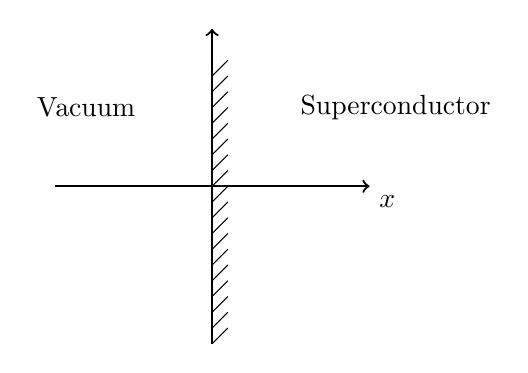
\begin{tikzpicture}[scale = 2]
\draw[thick, ->] (0,1) to (2,1);
\draw[thick, ->] (1,0) to (1, 2);
\foreach \y in {0,0.1,...,1.8} {
	\draw (1,\y) to (1.1, \y + 0.1);	
}
\node at (0.2,1.5) {Vacuum};
\node[anchor = west] at (1.5,1.5) {Superconductor};
\node[anchor = north west] at (2,1) {$x$};
\end{tikzpicture}
\caption{Semi-infinite superconductor}
\label{fig:semi_infinite_superconductor}
\end{figure}
Here, $\vb A = \vb A(x)$. At $x=0: \vb A(x=0) = \vb A_0$.
\begin{align} 
\dv[2]{\vb A}{x} &= \dfrac{1}{\lambda^2}\vb A  \\[2ex]
\implies \vb A(x) &= \vb A_0(x)\e^{-\frac{x}{\lambda}} \\[2ex]
\vb B(x) &= \curl{\vb A}
\end{align}
$B_i = \ep_{ijl}\partial_j A_l$. $j = x(=1)$ since there is only $x$-dependence. 
\begin{align*} 
B_y &= \ep_{213}\partial_x A_z =-\partial_xA_z = \frac1\lambda A_{0z}\e^{\frac{-x}{\lambda}} \\
B_z &= \ep_{312}\partial_x A_y =+\partial_xA_y = - \frac1\lambda A_{0y}\e^{\frac{-x}{\lambda}}
\end{align*}
Thus, 
\begin{equation} 
\vb B(x) = \vb B_0\e^{\frac{-x}{\lambda}}.
\end{equation}

\begin{figure}
	\centering
	\begin{tikzpicture}[scale = 0.75]
\begin{axis}[
axis lines = center,
x label style={ at={(axis description cs:1,0.05)}, anchor = west},
y label style={at={(axis description cs:0.45,1)},anchor=south},
ticks = none,
xlabel = $\Large x$,
ylabel = $\Large \vb B(x)$,
ymax = 1.3,
xmin =-1,
xmax=3
]

\addplot[thick,
domain=0:2, 
samples=100, 
color=blue]{exp(-x)};


\draw[->, thick] (axis cs:-0.3,0.3) to (axis cs:-0.3,0.9);
\node[anchor=east] at (axis cs:-0.3,0.6) {$\vb B_0$};
\node[anchor = south west] at (axis cs:0.6,0.5) {\Huge $\sim \e^{-\frac{x}{\lambda}}$};


\pgfplotsinvokeforeach{0,0.1,...,1.8} {
	\coordinate(a) at (axis cs:0,#1);
	\draw (a) -- ($(a) +(axis direction cs:0.1,0.1)$);	
};



\end{axis}
\end{tikzpicture}
\end{figure}
Now we see the physical meaning of $\lambda$: It is a characteristic length for how far a magnetic field penetrates a superconductor. It is referred to as the \underline{London penetration length.}
Thus, a magnetic field only exists withing a layer of thickness $\lambda$ from the surface of the superconductor. There is no magnetic field in the bulk of the superconductor. This is the Meissner-effect.
\begin{tcolorbox}[center, width = 0.5\textwidth]
	\centering
	Meissner-effect : $\lambda^{-1} >0$. \\[2ex]
	No Meissner-effect: $\lambda^{-1} = 0$. 
\end{tcolorbox}

The expression for $\lambda$ is
\begin{equation}
	\lambda = \left( \frac{m}{\mu_0n_s\left( e^* \right)^2} \right)^\frac{1}{2},
\end{equation}
a magnetic penetration length. $\lambda^{-1} > 0 $ if and only if $n_s >0$. $\lambda^{-1}=0$ otherwise. 
\underline{How does $n_s$ relate to $\Delta_k^\dagger$?}
$\Delta_k^\dagger$ originates with $b_k^\dagger = \ev{c_{-k\downarrow}c_{k\uparrow}}^\dagger$ which is the expectation value of the creation operator of a Cooper pair. Fourier-transformed to real-space it is the wavefunction $\psi(\vb r)$ of a Cooper-pair. $n_s \sim |\psi|^2$, thus $n_s \ne 0$ if and only if $\Delta_k\ne0$.\footnote{Says iff $\Delta_k = 0$ in the notes, which doesn't seem right.s}
Thus the onset of $\Delta_k$ for $T<T_C$ also means the onset of the Meissner-effect. 
\begin{tcolorbox}[center, width = 0.6\textwidth]
The onset of $\Delta_k$ at $T<T_C$ explains:
\begin{enumerate}[i)]
	\item loss of resistivity $\rho(T)$
	\item onset of Meissner-effect
\end{enumerate}
\end{tcolorbox}  